	\documentclass[10pt,oneside]{CBFT_book}
	% Algunos paquetes
	\usepackage{amssymb}
	\usepackage{amsmath}
	\usepackage{graphicx}
% 	\usepackage{libertine}
% 	\usepackage[bold-style=TeX]{unicode-math}
	\usepackage{lipsum}

	\usepackage{natbib}
	\setcitestyle{square}

	\usepackage{polyglossia}
	\setdefaultlanguage{spanish}
	



	\usepackage{CBFT.estilo} % Cargo la hoja de estilo

	% Tipografías
	% \setromanfont[Mapping=tex-text]{Linux Libertine O}
	% \setsansfont[Mapping=tex-text]{DejaVu Sans}
	% \setmonofont[Mapping=tex-text]{DejaVu Sans Mono}

	%===================================================================
	%	DOCUMENTO PROPIAMENTE DICHO
	%===================================================================

\begin{document}

% =================================================================================================
\chapter{Suma de momentos angulares}
% =================================================================================================

% =================================================================================================
\section{Armónicos esféricos como matrices de rotación}
% =================================================================================================

Se pueden hallar autoestados de dirección $\Ket{\hat{n}}$ rotando el $\Ket{\hat{z}}$,
\[
	\hat{n} = \mathcal{D}(R) \Ket{\hat{z}}
\]

\begin{figure}[!htb]
	\begin{center}
	\includegraphics[width=0.25\textwidth]{images/teo2_12.pdf}
	\end{center}
	\caption{.}
\end{figure} 
Necesitamos aplicar $\mathcal{D}(R)=\mathcal{D}(\alpha=\varphi,\beta=\theta,\gamma=0)$
\[
	\Ket{\hat{n}} = \sum_{m,\ell} \mathcal{D} (R) \Ket{\ell,m}\Braket{\ell,m|\hat{z}}
\]
\[
	\Braket{\ell,m'|\hat{n}} = \sum_{m,\ell} \Braket{\ell,m'|\mathcal{D} (R)| \ell,m}\Braket{\ell,m|\hat{z}}
\]
pero como la $\mathcal{D}(R)$ no conecta $\ell$ diferentes, se tiene 
\[
	\Braket{\ell,m'|\hat{n}} = \sum_{m} \mathcal{D}_{m'm}^\ell(R) \Braket{\ell,m|\hat{z}}	
\]
\[
	Y_\ell^{m'*}(\theta,\varphi) = \sum_m \mathcal{D}_{m'm}^\ell(R) Y_\ell^{m*} (\theta=0,\varphi \text{indet})
\]
pero como $\theta=0$ , $Y_\ell^m = 0$  con $m\neq 0$ se tiene 
\[
	\Braket{\ell,m|\hat{z}} = Y_\ell^{m*} (\theta=0,\varphi \text{indet}) \delta_{m0}
\]
\[
	\Braket{\ell,m|\hat{z}} = \sqrt{ \frac{2\ell +1}{4\pi} } \delta_{m0}
\]
\[
	Y_\ell^{m'*}(\theta,\varphi) = \sqrt{ \frac{2\ell +1}{4\pi} }
	\mathcal{D}_{m'0}^\ell (\alpha=\varphi,\beta=\theta,\gamma=0)
\]
la matriz de rotación en este caso es un armónico esférico.

La $\Psi$ tiene la misma simetría que el potencial.

% =================================================================================================
\section{Suma de momentos angulares}
% =================================================================================================

Sea un estado con valor $J$ máximo, entonces
\[
	J_z \Ket{j,j} = j\hbar \Ket{j,j} \qquad \qquad 
	J^2 \Ket{j,j} = j (j+1) \hbar^2 \Ket{j,j}
\]

Y se ve que si $j$ es muy grande, $J_z = j\hbar$ y $|j| = \sqrt{j(j+1)} \hbar$ están muy cerca.
Casi todo el $|j|$ está en $\zver$.


Clásicamente con $j\to\infty$ veremos que $J_x, J_y$ son casi nulos y es casi todo $J_z$.
El problema es que dada la incerteza en $J_x, J_y$ no puedo sumar todos los momentos $J_x + J_y + J_z $.
Este desconocimiento no es tan terrible por la cuantización de los momentos. En mecánica clásica un
desconocimiento de esta índole traería consecuencias desastrosas.

Es importante sumar momentos angulares para hacer cuentas como $\vb J = \vb L + \vb S$, o en ciertos 
cálculos de física nuclear.

\notamargen{Dos momentos de spín $1/2$}

Sean dos estados de spín $1/2$, donde es $S=1/2$ y definimos
\[
	\vb{S} = \vb{S}_1 + \vb{S}_2 \equiv 
	\vb{S}_1 \otimes \mathbb{1}_2 + \mathbb{1}_1\otimes \vb{S}_2,
\]
donde la identidad implica no realizar cambios sobre un estado particular.
En cada espacio valen las relaciones usuales de conmutación 
\[
	[ S_{1/2i},S_{1/2j}] = i\hbar\epsilon_{ijk}S_{1/2k}, \qquad  [S_{1i},S_{2j}] = 0
\]
donde el último indica que operadores de espacios diferentes conmutan.

Clasificaremos los autoestados como $\Ket{s_1,m_1}, \Ket{s_2,m_2}$ de modo que
\[
	S_1^2 \Ket{s_1,m_1} = s_1 ( s_1 + 1 ) \hbar^2 \Ket{s_1,m_1} \qquad 
	{S_2}_z \Ket{s_2,m_2} = m_2 \hbar \Ket{s_2,m_2}
\]

Un estado general se puede escribir según 
\[
	\Ket{S_1,m_1} \otimes \Ket{S_2,m_2} \equiv \Ket{S_1, S_2;m_1,m_2}
\]
dándose que $S_1^2, S_2^2, S_{1z}, S_{2z}$ conmutan entre sí. Por ello podemos acoplar los 
cuatro índices como se hizo arriba. 
\notamargen{Explicarlo mejor.}

Dado que estamos en el caso de spin $1/2$ tenemos cuatro estados posibles 
\be
	\Ket{++} \qquad \Ket{+-} \qquad \Ket{-+} \qquad \Ket{--}
	\label{base1}
\ee

Esto no nos da información del spin suma de las dos partículas, sino del spin de cada una 
de ellas. Si se quiere saber $S^2 = S_1^2 + S_2^2, S_z=S_{1z} + S_{2z}$ otro examen tiene que
ser hecho.
Nótese que $ [S^2, S_{2z}] \neq 0  $ puesto que $ (S_1+S_2)^2 = S_1^2 + S_2^2 + 2 \pe{S_1}{S_2}$.

Se puede elegir otro COCC como $S_1^2, S_2^2, S^2, S_z$ base inteligente para clasificar la
suma de los momentos. Así tendremos $\Ket{S_1, S_2 ; S, m}$ donde el tercero y cuarto están
asociados a $S^2$ y $S_z$, respectivamente. Entonces
\[
	S^2\Ket{S_1, S_2 ; S, m} = s(s+1)\hbar^2 \Ket{S_1, S_2 ; S, m} 
\]
\[
	S_z \Ket{S_1, S_2 ; S, m} = m \hbar \Ket{S_1, S_2 ; S, m}
\]

Combinando dos estados de spin $1/2$ surgen
\begin{multline}
	\{ \Ket{1/2,1/2,1,1} , \;  \Ket{1/2,1/2,1,0}, \: \Ket{1/2,1/2,1,-1} \}
	\qquad \text{ triplete } [s=1]
	\\
	\{ \Ket{1/2,1/2,0,0} \}
	\qquad \text{ singlete } [s=1/2]
	\label{base2}
\end{multline}

Tenemos escritos los estados en dos bases \eqref{base1} y \eqref{base2}, siendo la primera muy
sencilla pero menos útil que la segunda. Tratemos de pasar entre bases. Vemos que
\[
	\Ket{++} = \Ket{S_1=1/2, S_2=1/2, m_1=1/2, m_2=1/2},
\]
desde lo cual podemos ve algo por inspección.
[sigue acá info entretejida con lo anterior]

Hay cuatro estados
\[
	\begin{matrix} S_1 \quad S_2 \quad\quad m_1 \quad m_2 \end{matrix}
\]
\[
	\begin{matrix}
	&\Ket{1/2, 1/2 ; \phantom{-}1/2, \phantom{-}1/2} \\
	&\Ket{1/2, 1/2 ; \phantom{-}1/2, -1/2} \\
	&\Ket{1/2, 1/2 ; -1/2, -1/2} \\
	&\Ket{1/2, 1/2 ; -1/2, \phantom{-}1/2}
	\end{matrix}
\]	
\[	
	\begin{matrix} S_1 \quad S_2 \quad\quad S_{1z} \quad S_{2z}  \end{matrix}
\]
que corresponden a los operadores $S_ 1^2, S_2^2, S_{1z}, S_{2z}$ que conmutan (son un CCOC).

Podemos elegir otras base de operadores que comutan que será: $S_ 1^2, S_2^2, S, S_{z}$, de modo
que el estado general será
\[
	\Ket{S_1, S_2;S,m}
\]
Así tendremos
\[
	\begin{matrix} \qquad\qquad S_1 \quad S_2 \quad S \quad m \end{matrix}
\]
\[
	\begin{matrix}
	\text{Triplete}\begin{cases}	
	&\Ket{1/2, 1/2 \; ; \; 1, \phantom{-}1} \\
	&\Ket{1/2, 1/2 \; ; \; 1, \phantom{-}0} \\
	&\Ket{1/2, 1/2 \; ; \; 1, -1} \\
	\end{cases}
	\\
	\text{Singlete}\begin{cases}
	&\Ket{1/2, 1/2 \; ; \; 0, \phantom{-}0} \\
	\end{cases}		
	\end{matrix}	 
\]	
\[	
	\begin{matrix} \qquad\qquad S_1^2 \quad S_2^2 \quad S^2 \quad S_z  \end{matrix}
\]
y recordemos que $m_1+m_2=m$ y $s_1+s_2=s$
\[
	S^2 = (S_1 + S_2)^2  = S_1^2 + S_2^2 + 2\vb{S}_1\cdot\vb{S}_2 \qquad 
	S^2_z = (S_{1z} + S_{2z})^2  = S_{1z}^2 + S_{2z}^2 + 2S_{1z}\cdot S_{2z}
\]

Dada la repetición de $S_1,D_2$ se suelen identificar a las bases solamente 
\[
	\begin{cases}
	\{ \Ket{m_1,m_2} \} \\
	\{ \Ket{S,m} \}
	\end{cases}
\]
Además la base $\{ \Ket{m_1,m_2}\}$ se puede poner como 
\[
	+ \equiv + 1/2 \qquad\qquad - \equiv - 1/2
\]

\subsection{Cambio entre bases}

Podemos hallar a ojo que 
% \[
% 	\cdot \Ket{++} = \Ket{1,1} \qquad \cdot \Ket{--} = \Ket{1,-1}
% \]
\begin{itemize}
 \item $\Ket{++} = \Ket{1/2, 1/2; 1, 1} \equiv \Ket{1,1}$
 \item $\Ket{--} = \Ket{1,-1}$
\end{itemize}
porque acoplamos máximos de cada partícula lo que dará el máximo o mínimo en la suma; 
la única forma de tener $m=1$ es con los dos spines up y la única forma de tener $m=-1$ 
es con los dos spines down.

Se hallan los otros con el operador de bajada
\[
	S_- \equiv S_{1-} + S_{2-}
\]
y si descompongo $S_-$ en $S_{1-}$ y $S_{2-}$ para operar en $\Braket{s,m}$ se tiene 
\begin{multline*}
	S_- \Ket{++} = S_{1-}\Ket{++} + S_{2-}\Ket{++} = \\
	S_{1-}\otimes\mathbb{1}_2\Ket{++} + \mathbb{1}_1\otimes S_{2-}\Ket{++} = 
	\hbar\Ket{-+} + \hbar\Ket{+-} 
\end{multline*}
y ahora si opero con $S_-$,
\[
	S_-\Ket{11} = \sqrt{2} \hbar \Ket{10}
\]
\begin{itemize}
	\item $\Ket{10} = \frac{1}{\sqrt{2}}( \Ket{-+} + \Ket{+-} ) $
\end{itemize}

Luego, queda por hallar $\Ket{00}$, que será algo como 
\[
	\Ket{00} = a \Ket{+-} + b\Ket{-+}
\]
y puedo usar ortonormalidad 
\[
	\Braket{10|00} = 0 = \frac{a}{\sqrt{2}} + \frac{b}{\sqrt{2}} \qquad \text{con} \; |a|^2 + |b|^2 = 1
\]
\begin{itemize}
	\item $\displaystyle \Ket{00} = \frac{1}{\sqrt{2}}( \Ket{+-} - \Ket{-+} ) $
\end{itemize}

Se puede ver entonces que son simétricos los miembros del triplete y antisimétricos los del
singlete porque al intercambiar $+$ con $-$ en las expresiones cambian los valores o no cambian:
ahí está la simetría.
Usualmente interesa la matriz del cambio de base y sus coeficientes (los de Clebsh-Gordan).


\subsection{Teoría formal de suma de momentos angulares}

Sea de sumar dos momentos angulares $J_1, J_2$. Las relaciones de conmutación son
\[
	[J_{1i},J_{1j}] = i\hbar \varepsilon_{ijk}J_{1k} \qquad 
	[J_{2i},J_{2j}] = i\hbar \varepsilon_{ijk}J_{2k} \qquad
	[J_{1k},J_{2l}] = 0
\]
\[
	\vb{J} = \vb{J}_1 \otimes \mathbb{1}_2 + \mathbb{1}_1\otimes \vb{J}_2 
	\equiv \vb{J}_1 + \vb{J}_2
\]
\[
	[J_i, J_j] = i\hbar\epsilon_{ijk}J_k
\]
donde en el último renglón cada $J$ actúa en el espacio en donde {\it vive}.
El momento total \vb{J} cumple que 
\[
	J^2 =  J_1^2 + J_2^2 + 2J_1J_2 \qquad 
	J^2 =  J_1^2 + J_2^2 + 2J_{1z}J_{2z} + J_{1+}J_{2-} + J_{1-}J_{2+}
\]
donde vemos que 
\[
	[J^2_{1/2},J^2] = 0 \qquad [J_z,J^2] = 0 \qquad [J^2_{1/2},J_{1/2,z,+,-}] = 0
\]
pero 
\[
	[ J^2 , J_{1z}] \neq 0  \qquad \qquad [ J^2 , J_{2z}] \neq 0
\]

Esto deja dos opciones para elegir un CCOC

\begin{center}
\begin{tabular}{|c|c|}
\hline 
$J_1^2, J_2^2, J_{1z}, J_{2z}$ & $J_1^2, J_2^2, J^2, J_{z}$ \\
& \\
$\Ket{j_1,j_2;m_1,m_2}$ & $\Ket{j_1,j_2;j,m}$ \\
& \\
base desacoplada & base acoplada \\
\hline
\end{tabular}
\end{center}
\notamargen{Tenía anotado que en la base acoplada se suele
abreviar no expresando los dos índices comunes $j_1,j_2$ en el ket.}

Se puede pasar de una base a otra con una identidad $\mathbb{1}$ apropiada
\[
	\Ket{j_1,j_2;j,m} = \sum_{m_1,m_2} \Ket{j_1,j_2;m_1,m_2}\Braket{j_1,j_2;m_1,m_2|j_1,j_2;j,m}
\]
\[
	1. \; \Ket{j_1,j_2;j,m} = \sum_{m_1,m_2} C_{m_1m_2}^j \Ket{j_1,j_2;m_1,m_2}
\]
con la restricción de que $-j_1 \leq m_1 \leq j_1$ y $-j_2 \leq m_2 \leq j_2$.
Los $C_{m_1 m_2}^j$ son los coeficientes de Clebsh-Gordan. 
Los coeficientes inversos son paridos desde 
\[
	\Ket{j_1,j_2;m_1,m_2} = \sum_{j,m} \Ket{j_1,j_2;j,m}\Braket{j_1,j_2;j,m|j_1,j_2;m_1,m_2}
\]
\[
	2. \; \Ket{j_1,j_2;m_1,m_2} = \sum_{j,m} C_{m_1m_2}^{j*}\Ket{j_1,j_2;j,m}
\]
con $-j \leq m \leq j$ y con $j\to\infty$, porque la sumatoria en $j$ es infinita, aunque se verá
que muchos son nulos.
\notamargen{En la página 51 de la carpeta bajo ``caso general de suma de J'' tengo anotadas algunas
expresiones de resumen de la práctica que deberían repetir esto.}
En 2 la $\sum$ sería en $j\to\infty$, pero veamos la relacion que hace algunos $C_{m_1 m_2}^j=0$. 
Ante todo abreviaremos suprimiendo los índices $j_1,j_2$ con lo cual 
\[
	C_{m_1m_2}^{j} = \Braket{m_1,m_2|j,m}
\]
A partir de
\[
	(J_{z} - J_{1z} - J_{2z})\Ket{j,m} = (m\hbar - J_{1z} - J_{2z})\Ket{j,m} = 0
\]
se ve que
\[
	\Braket{m_1,m_2|(J_{z} - J_{1z} - J_{2z})|j,m}= 0, 
\]
\[
	\hbar(m-m_1-m_2)\Braket{m_1,m_2|j,m} = \hbar(m-m_1-m_2) C^j_{m_1 m_2} = 0
\]
entonces para que $C^j_{m_1 m_2}$ sea no nulo se necesita $m = m_1 + m_2$.
Esta condición restringe los coeficientes un poco.
% \[
% 	\Braket{m_1,m_2| j,m} \neq 0 \iff m = m_1 + m_2
% \]

A su vez, en la suma de $J_1$ y $J_2$ resultan los $j$ acotados por una desigualdad triangular 
\[
	|j_1 - j_2| \leq j \leq j_1 + j_2
\]
Notemos que para $j_1 \to 2 j_1 + 1, j_2 \to 2j_2 + 1$; luego tendemos combinaciones por 
$(2 j_1 + 1)(2 j_2 + 1)$ en la base desacoplada.

Asimismo los $C_{m_1 m_2}^j$ se toman reales, entonces 
\[
	C_{m_1m_2}^{j*} = C_{m_1m_2}^{j}
\]
y juntando todo se tiene 
\[
	\Braket{m_1,m_2|j,m} \neq 0	\iff  m = m_1 + m_2,
\]
o lo que es equivalente
\[
	\Braket{j,m|m_1,m_2} \iff |j_1 - j_2| \leq j \leq j_1 + j_2.
\]

En la base desacoplada, la restricción limita el no llegar al infinito.
Ambas bases tienen la misma dimensión si sumamos entre los límites dados
\[
	\sum_{j=|j_1-j_2|}^{ j_1 + j_2 } \: 2j+1 = (2j_1 + 1)(2j_2 + 1).
\]

Recordemos que cada $j$ tiene $2j+1$ estados posibles (los $m$ correspondientes a 
cada $j$) ($|m|\leq j$). 

Esta es una demostración más o menos deficiente. Podemos volver al ejemplo de 
$j_1 = 1/2$ y $j_2=1/2$ considerando
\[
	\text{ j } \; \frac{1}{2} \otimes \frac{1}{2} = 1 \oplus 0 
\]
\[
	\text{ dim } \; {2} \otimes {2} = 3 \oplus 1
\]

Cualesquiera cosas que cumplan el álgebra del momento angular permiten hacer una
analogía es un espacio símil.
\notamargen{Esto es un claim muy importante de group theory.}

\begin{ejemplo}{\bf Partículas}

Sean dos partículas con $j_1=2$ y $j_2=1$ que tendrán 5 y 3 estados posibles. El número total
de estados posibles será quince. Veamos todas las combinaciones posibles en la base
$(m_1,m_2)$ que se pueden agrupar en la tabla siguiente

\begin{center}
\begin{tabular}{cccccccc}
$m$ & $3$ & $2$ & $1$ & $0$ & $-1$ & $-2$ & $-3$ \\
\hline
$(m_1,m_2)$ & $(2,1)$ & $(1,1)$ & $(0,1)$ & $(-1,1)$ & $(2,1)$ &  & \\
$(m_1,m_2)$ &  & $(2,0)$ & $(1,0)$ & $(0,0)$ & $(-1,0)$ & $(-2,0)$ &  \\
$(m_1,m_2)$ &  &  & $(2,-1)$ & $(1,-1)$ & $(0,-1)$ & $(-1,-1)$ & $(-2,-1)$ \\
\hline
\end{tabular}
\end{center}

Luego, se tienen
\begin{eqnarray*}
	m = 3,2,1,0,-1,-2,-3 \qquad  & j=3 \qquad & \text{ 7 estados (septete)} \\
	m = 2,1,0,-1,-2 \qquad  & j=2 \qquad & \text{ 5 estados (quintuplete)} \\
	m = 1,0,-1 \qquad  & j=1 \qquad & \text{ 3 estados (triplete)} 
\end{eqnarray*}

Esto nos da los valores de $j$ que podemos alcanzar; pero no nos dice que los estados son ellos todos.
Así, $\Ket{j=3,m=2}$ se forma como combinación lineal de $(1,1)$ y $(2,0)$.
Me he construido de esta forma los multipletes $j=3, j=2, j=1$ y se puede generalizar.
Estuvimos haciendo
\[
	\text{ j } \; 2 \otimes 1 = 3 \oplus 2 \oplus 1 
\]
\[
	\text{ dim } \; {5} \otimes {3} = 7 \oplus 5 \oplus 3
\]

Queremos calcular los coeficientes de Clebsh-Gordan
\be
	\Ket{j_1,j_2;j, m} = \sum_{m_2=-j_2}^{j_2}\sum_{m_1=-j_1}^{j_1}
	\Ket{j_1,j_2; m_1, m_2} \: C_{m, m_2}^j
	\label{clebsh_gordan}
\ee
sumatorias sujeta a $m_1+m_2=m$.

Consideremos un caso sencillos: $j_1=1$ y $j_2 =3/2$ de modo que $j=5/2, 3/2, 1/2$.
Si sumamos $j_1=1, j_2=3/2$ tendremos 
\[
	\text{dim} =  2 \oplus 4 \oplus 6 = 3 \otimes 4 = 12
\]

Para hacer la cuenta \eqref{clebsh_gordan} tengo 12 coeficientes muchos de los cuales
serán nulos. Miramos de qué forma podemos llegar a $m_1 + m_2 = 3/2$, por ejemplo si
es que queremos formar el estado $\Ket{1, 3/2 ; 5/2, 3/2}$. Entonces, como
\[
	j_1 = 1 \to \left\{ 1,0,-1 \right\} \qquad 
	j_2 = \frac 3 2 \to \left\{ \frac{3}{2},\frac{1}{2}, -\frac{1}{2}, -\frac{3}{2} \right\}
\]
obtengo $3/2$ con $(0,3/2)$ y $(1,1/2)$ de manera que tendremos
\[
	C_{0 \: 3/2}^{5/2} \Ket{1 , 3/2 ; 0, 3/2} +
	C_{1 \: 1/2}^{5/2} \Ket{1 , 3/2 ; 1, 1/2}
\]

Como tenemos libertad de elegir fase para los coeficientes, elegimos que la matriz sea real
y como es unitaria por ser un cambio de base, será ortogonal.
El $\Ket{1,3/2;5/2,5/2}$ solo lo puedo alcanzar con los vectores paralelos sumados entre sí.
El coeficiente de Clebsh-Gordan del más alto vale uno porque es el único. A partir de este
puedo usar operadores de subida y de bajada para construirme los faltantes.\

Por ortonormalidad se tiene
\[
	\Braket{ j_1, j_2 ; m_1', m_2' } = \delta_{m_1' m_1}  \delta_{m_2' m_2}
\]
\[
	\sum_{j,m} \KB{ j_1, j_2 ; j, m }{ j_1, j_2 ; j, m }
\]
pero esta condición es fea y no la usaremos.
Es más conveniente esta otra
\[
	\Braket{j',m'|j,m} = \delta_{j'j}\delta_{m'm}
\]
\[
	\sum_{m_1,m_2} \Braket{j',m'|m_1,m_2}\Braket{m_1,m_2|j,m} = \delta_{j'j}\delta_{m'm}
\]
\[
	\sum_{m_1,m_2} \Braket{m_1,m_2|j,m}^2 = 1
\]
siendo esto último la ortonormalidad.

Nos podemos construir a partir de uno con una recurrencia. Partimos de
\[
	J_\pm \ket{j,m} = ( J_{1\pm} + J_{2\pm} ) \sum_{m_1',m_2'} \Ket{m_1',m_2'}\Braket{m_1',m_2'|j,m}
\]
\[
	\sqrt{(j\mp m)(j\pm m + 1)} \ket{j,m\pm 1} = \sum_{m_1',m_2'}\Braket{m_1',m_2'|j,m}  
	( J_{1\pm}\Ket{m_1',m_2'} + J_{2\pm}\Ket{m_1',m_2'} ) 
\]
y multiplicando por un bra $\Bra{m_1,m_2}$ la expresión anterior, se llega a la relación de recurrencia
\begin{multline*}
	\sqrt{(j\mp m)(j\pm m + 1)} \Braket{m_1,m_2|j,m\pm 1} = \\
	\sqrt{(j_1 \mp m_1 + 1 )(j_1 \pm m_1)} \Braket{m_1 \mp 1 ,m_2|j,m}  + \\
	\sqrt{(j_2 \mp m_2 + 1 )(j_2 \pm m_2)}  \Braket{m_1,m_2 \mp 1| j,m } 
\end{multline*}
que nos dice que necesito conocer dos coeficientes para conocer otro.
 
\end{ejemplo}
% \[
% 	j = 1/2, 3/2, 5/2 \qquad m_1 = -1,0,1
% \]
% \[
% 	j = -5/2,-3/2,-1/2,1/2, 3/2, 5/2 \qquad m_2 = -3/2,-1/2,1/2,3/2
% \]
% 
% Podemos ver a ojo que 
% \[
% 	\Ket{j=5/2,m=5/2} = \Ket{m_1=1,m_2=3/2}
% \]
% \[
% 	\Ket{j=5/2,m=-5/2} = \Ket{m_1=-1,m_2=-3/2}
% \]
% luego con el $J_=, J_-$ podemos construirnos los siguientes (utilizando ortonormalidad)


\section{Coeficientes de Clebsh-Gordan}

Habíamos probado ciertas condiciones parda los coeficientes de Clebsh-Gordan
\[
	\Ket{j_1,j_2;j,m} = \sum_{m_1,m_2} C_{m_1 m_2}^{j} \: \Ket{ j_1 j_2 m_1 m_2 }
\]
con $m_1 + m_2 = m$ y donde $j$ verifica $ j_1 + j_2 \geq j \geq | j_1 - j_2 |$.

Veamos un caso de sumar $\vb L + \vb S$ (momento angular más spin) en el caso de spin $1/2$.
Identificamos entonces $j_1 = \ell, m_1 = m_\ell, j_2 = 2 = 1/2$ y $m_2 = m_s = \pm 1/2$ 
Esto nos lleva a
\[
	|\ell - \frac 1 2 | \leq j \leq \ell + \frac 1 2
\]
y
\[
	j = \ell \pm \frac{1}{2} \quad \ell > 0 \qquad \qquad j = \frac 1 2 \quad \ell = 0
\]

La expresión de [1] nos dice simplemente que sumando spin más momento angular se tiene $\ell+1/2$ 
o $\ell - 1/2$ si están simétricos o antisimétricos. Veamos los coeficientes de Clebsh-Gordan que
no serán nulos,
Tendremos dos estados
\begin{multline*}
	\Ket{\ell + \frac 1 2, m } =
	\Braket{ m - \frac 1 2 \; \frac 1 2 | \ell + \frac 1 2 \; m } 
	\Ket{ m - \frac 1 2, \frac 1 2 } \\
	+
	\Braket{ m - \frac 1 2 \; -\frac 1 2 | \ell + \frac 1 2 \; m }
	\Ket{ m + \frac 1 2, -\frac 1 2 }
\end{multline*}
donde el braket del primer término es A y el del segundo es B.
\begin{multline*}
	\Ket{\ell - \frac 1 2, m } =
	\Braket{ m - \frac 1 2 \; \frac 1 2 | \ell - \frac 1 2 \; m } 
	\Ket{ m - \frac 1 2, \frac 1 2 } \\
	+
	\Braket{ m + \frac 1 2 \; -\frac 1 2 | \ell - \frac 1 2 \; m }
	\Ket{ m + \frac 1 2, -\frac 1 2 }
\end{multline*}
donde el braket del primer término es C y el del segundo es D.
\notamargen{Tiramos $j_1, j_2$ para simplificar la notación.}
Además se ve que no nulos serán $ m = m_1 + m_2 = m_\ell \pm 1/2 $ y  $m_1 = m \pm 1/2$.
Dado el caso que estamos tratando, $S$ solo tiene dos valores que dan $ m = m_1 + m_2 $. Los
coeficientes de Clebsh-Gordan vinculan los estados con $j = \ell \pm 1/2$ y $m$. Podemos poner
todo en una matriz
\[
	\ell - \frac{1}{2} \quad m \qquad \ell + \frac{1}{2} \quad m
\]
\notamargen{Acá hay que armar alguna cosa customizada para poner sobre los bordes de la matriz
la equivalencia de filas columnas (yo me entiendo).}
\[
	\begin{matrix} 
	m + \frac 1 2 & -\frac 1 2 \\
	\\
	m - \frac 1 2 & \frac 1 2
	\end{matrix}
	\begin{pmatrix}
		\; D & B \; \\
		\\
		\; C & A \;
	\end{pmatrix} 
	\equiv
	\begin{pmatrix}
		\cos\a & \sin\a \\
		\\
		-\sin\a & \cos\a
	\end{pmatrix}
\]

Por convención se toma coeficiente de $\sin\alpha > 0$. La equivalencia ha llegado a una matriz
ortogonal por la realidad de sus coeficientes. Calcularemos algún coeficiente
\[
	\cos \a = \Braket{ m - \frac 1 2, \frac 1 2 | \ell + \frac 1 2, m }.
\]

Hay un modelo gráfico para la recurrencia. Podemos graficar ahora

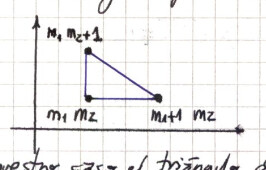
\includegraphics[width=0.40\textwidth]{images/fig_ft2_recurrencia_1.jpg}
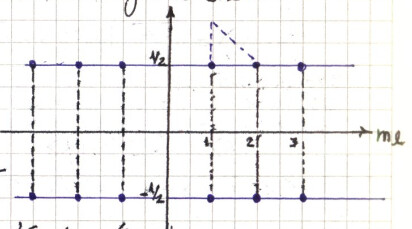
\includegraphics[width=0.40\textwidth]{images/fig_ft2_recurrencia_2.jpg}

En nuestro caso el triángulo d recurrencia no conecta hacia arriba porque para spin solo tengo
$+ 1/2$ o $-1/2$, con lo cual no tengo el trío sino un dúo de coeficientes.
Trabajando encontramos que
\[
	\Braket{ m - \frac 1 2, \frac 1 2 | \ell + \frac 1 2, m } =
	\sqrt{\frac{ ( \ell + m + 1 / 2 ) }{ \ell + m + 3 / 2 }} \:
	\Braket{ m + \frac 1 2, \frac 1 2 | \ell + \frac 1 2, m + \frac 1 2 }
\]

Esta relación puede aplicarse hasta $m+1/2 \to \ell$. Entonces llegamos a
\[
	\Braket{ m - \frac 1 2, \frac 1 2 | \ell + \frac 1 2, m } =
	\sqrt{\frac{ ( \ell + m + 1 / 2 ) }{ 2 \ell + 1 }} \:
	\Braket{ \ell, \frac 1 2 | \ell + \frac 1 2, \ell + \frac 1 2 }
\]

Llegamos a los máximos valores (todo en $\zver$ el momento angular, todo en $\zver$ el spin $S$)
con lo cual debe dar el máximo y entonces el coeficiente debe dar uno $\Braket{\ell,1/2| \ell+1/2,\ell+1/2} = 1$.
Identificamos
\[
	\sqrt{\frac{ ( \ell + m + 1 / 2 ) }{ 2 \ell + 1 }} \equiv \cos\a
	\qquad \qquad 
	\sqrt{\frac{ ( \ell - m + 1 / 2 ) }{ 2 \ell + 1 }} \equiv \sin\a
\]

donde siempre podemos fijar inicialmente la fase para que sea real.
Es útil en el acoplamiento spin-órbita. Allí teníamos
\[
	\pe{L}{S} = \frac{1}{2} ( J^2 - L^2 - S^2 )
\]
\[
	\pe{L}{S} \Ket{\ell,s, j, m} = 
	\frac{\hbar^2}{2} \left[ 
	j(j+1) - \ell(\ell+1) - s(s+1)
	\right] =
	\begin{cases}
		\frac{\ell \hbar^2}{2} \quad j = \ell + \frac{1}{2} \\
		\\
		-\frac{ ( 1 + \ell ) \hbar^2}{2} \quad j = \ell - \frac{1}{2}
	\end{cases}
\]

Sea una cosa con $\ell=1, s=1/2$ lo que significa  $ 1 \otimes 1/2 = 3/2 \oplus 1/2$ o en términos
de dimensiones $ 3 \otimes 2 = 4 \oplus 2 $.
Escribo un estado en términos de la base mostrada
\[
	\Ket{ \frac 3 2 , \frac 3 2 } = \Ket{ 1 , \frac 1 2 }
\]
\[
	\Ket{ \frac 3 2 , \frac 1 2 } = 
	\sqrt{\frac{1}{3}} \: \Ket{ 1 , -\frac 1 2 } + \sqrt{\frac{2}{3}} \: \Ket{ 0 , \frac 1 2 }
\]

\notamargen{El término $\pe{L}{S}$ aparece en el lagrangiano de interacción nuclear.}

\subsection{Uso de la tabla de Clebsh-Gordan}


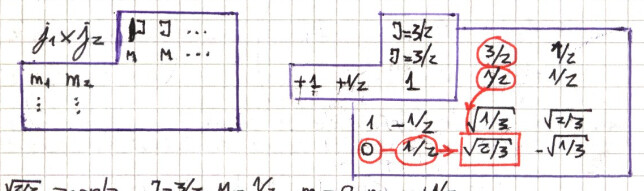
\includegraphics[width=0.60\textwidth]{images/fig_ft2_clebsh_gordan_table.jpg}

El primero y el final siempre valen uno porque acoplan estados máximos o mínimos.


El $\sqrt{2/3}$ acopla $j=3/2, M=1/2, m_1=0, m_2 =1/2$. Consideremos un ejemplo $2 \times 3/2$ lo cual 
corresponde a $j=7/2, 5/2, 3/2, 1/2$.
\[
	\Ket{\frac 7 2 , \frac 3 2} = \sqrt{\frac{2}{7}} \Ket{0,\frac 3 2} +
	\sqrt{\frac{4}{7}} \Ket{0,\frac 1 2} + \sqrt{\frac{1}{7}} \Ket{2,-\frac 1 2}
\]
Miro en la tabla $2\times 3$.
\notamargen{Es buena pensar qué CL general produce el $\Ket{7/2,3/2}$.}

Queremos ver cuándo un operador cumple propiedades vectoriales. En mecánica clásica teníamos la transformación
ante rotacionaes $V_i \to \sum_j R_{ij} V_j$ de modo que como $\Ket{\a} \to D(R)\Ket{\a}$ entonces
\[
	\Braket{\a|\mathcal{O}|\a} \to \Braket{\a | D^\dagger(R) \mathcal{O} D(R)|\a} 
	\qquad \qquad [\mathcal{O},J] =0
\]

Supongamos una rotación infinitesimal, se escribe el $D(R) = \mathbb{1} - i \epsilon \vb J \cdot \nver / \hbar$
\[
	D^\dagger \mathcal{O} D = \left( 1 + \frac{i\epsilon \vb J \cdot \nver}{\hbar}\right) 
	\mathcal{O} \left( 1 - \frac{i\epsilon \vb J \cdot \nver}{\hbar}\right) =  \mathcal{O}
	+ \frac{i\epsilon}{\hbar} [\mathcal{O},\vb J \cdot \nver] + \mathcal{O}(\epsilon^2)
\]
\notamargen{Qué mal elegido justo que usamos orden $\mathcal{O}$ y un operador $\mathcal{O}$.}

Al tomar valor medio resultará $\mathcal{O}$. Un operador vectorial en mecánica cuántica quedará definido
al hacer el traspaso
\[
	\Braket{\a|V_i|\a} \to \Braket{\a| D^\dagger V_i D |\a} \equiv \sum_j R_j \Braket{\a|V_j|\a}
\]
\[
	D^\dagger V_i D = \sum_j R_j V_j
\]
que es un operador vectorial, donde
\[
	V_i + \frac{\epsilon}{i\hbar} [V_i, \vb J \cdot \nver ] = \sum_j R_j V_j
\]
\[
	\begin{pmatrix}
		1 	&	-\epsilon	&	0 \\
		\epsilon &	1	&	0 \\
		0 	&	0	&	1 
	\end{pmatrix}
	\begin{pmatrix}
		V_x \\
		V_y \\
		V_z
	\end{pmatrix}
\]
\[
	V_x + \frac{\epsilon}{i\hbar} [ V_x, J_z ] = V_x - \epsilon V_y
\]
\[
	V_y + \frac{\epsilon}{i\hbar} [ V_y, J_z ] = V_y + \epsilon V_x
\]
\[
	V_z + \frac{\epsilon}{i\hbar} [ V_z, J_z ] = V_z
\]
Entonces, un operador es un operador vectorial cuando verifica que
\[
	[V_i, J_j] = i \hbar \epsilon_{ijk} V_k \qquad 
	[J_i, J_j] = i \hbar \epsilon_{ijk} J_k
\]
y vemos que $J$ es una especie de patrón de operadores vectoriales.

\begin{ejemplo}{\bf Ejercicio 1}
 
Consideremos $s=1/2, \ell=1$ con $\Ket{\ell,s,m_\ell,m_s}$ sujetos a $|\ell-s| \leq j \leq \ell + s$.
Tenemos que elegir $1,1/2$ para formar el $3/2$ lo que implica que $ j \leq 3/2$ y $m_{\text{max}}=3/2$.
\[
	\Ket{3/2, 3/2} = \Ket{1,1/2,1,1/2}
\]
Usemos $J_- = L_- + S_-$
\[
	J_- \Ket{3/2, 3/2} = \hbar \sqrt{3} \Ket{3/2,1/2}
\]
y
\[
	L_- S_- \Ket{1,1/2,1,1/2} = \hbar ( \sqrt{2} \Ket{1,1/2,0,1/2} + 1/\sqrt{3} \Ket{1,1/2,1,-1/2} )
\]
y luego
\[
	\Ket{3/2, 1/2} = \sqrt{2/3} \Ket{1,1/2,0,1/2} + 1/\sqrt{3} \Ket{1,1/2,1,-1/2}
\]

Usamos la tabla para hallar los otros coeficientes
\[
	\Ket{3/2, -1/2} = \sqrt{2/3} \Ket{1,1/2,0,-1/2} + 1/\sqrt{3} \Ket{1,1/2,-1,1/2}
	\qquad 
	\Ket{3/2, -3/2} = 1 \Ket{1,1/2,-1,-1/2}
\]

Faltan dos estados, y sale caminando mirando la tabla o completando por ortogonalidad que es el
\[
	\Ket{1/2, 1/2} = \sqrt{2/3} \Ket{1,1/2,-1,1/2} - \sqrt{1/3} \Ket{1,1/2,0,1/2}
\]
(este es lo mismo que multiplicarlo todo por $-1$) y
\[
	\vm{L_z} = 2/3 \hbar \qquad \vm{S_z} = -\hbar/6 \qquad \vm{J_z} = \hbar/2
\]
 
\end{ejemplo}


\begin{ejemplo}{\bf Ejercicio 6}
 
Tenemos dos partículas de spin $1/2$ 

Parte a)
\[
	\text{ Sujeto A } \longrightarrow (S_{1x}, S_{1y}, S_{1z})
\]
\[
	\text{ Sujeto B } \longrightarrow (S_{2x}, S_{2y}, S_{2z})
\] 
y el nulo es
\[
	\Ket{0,0} = \frac{1}{\sqrt{2}} ( \Ket{ 1/2, 1/2 ; 1/2, -1/2 } - \Ket{ 1/2, 1/2 ; -1/2, 1/2 })
\]

La probabilidad de $S_{1z} = \hbar/2$ es $1/2$, lo cual se ve a ojo.
Pero la otra probabilidad no es tan fácil. Conviene escribir $S_x$ en combinación lineal de
autoestados de $S_z$
\[
	\Ket{1/2, 1/2, 1/2, -1/2} = \frac{1}{\sqrt{2}}
	( \Ket{ 1/2, 1/2, m_x = 1/2, -1/2 } + \Ket{ 1/2, 1/2, m_x = -1/2, -1/2 } )
\]
\[
	\Ket{1/2, 1/2, -1/2, 1/2} = \frac{1}{\sqrt{2}}
	( \Ket{ 1/2, 1/2, m_x = 1/2, 1/2 } - \Ket{ 1/2, 1/2, m_x = -1/2, 1/2 } )
\]
\[
	\Ket{ 1/2 1/2 } \otimes \Ket{ 1/2 -1/2 }
\]

Son los cuatro ortogonales (este es el problema)
\begin{multline*}
	\Ket{ 0  0 } = \frac{1}{2}
	\left( \Ket{ 1/2, 1/2, m_x = 1/2, -1/2 } +
	\Ket{ 1/2, 1/2, m_x = -1/2, -1/2 } + \right. \\
	\left. \Ket{ 1/2, 1/2, m_x = 1/2, 1/2 } -
	\Ket{ 1/2, 1/2, m_x = -1/2, 1/2 }
	\right) 
\end{multline*}
y
\[
	P( S_x = \hbar/2 ) = \frac{1}{2}.
\]

Para la parte b) consideramos
\[
	\Ket{ 0 0 } = \frac{1}{\sqrt{2}} 
	( \Ket{1/2, 1/2 ; 1/2, -1/2} - \Ket{1/2, 1/2 ; -1/2, 1/2} )
\]
y como $B$ mide $S_{2z} = \hbar/2$ se tiene
\[
	\Ket{\Psi}_{\text{DM}} = \Ket{1/2, 1/2 ; -1/2, 1/2}
\]
pero $A$ mide $-\hbar/2$ de tal manera que $P(S_{1z}=-\hbar/2)=1$ puesto que $A$ seguro
mide $-\hbar/2$.

Si las partículas fueron separadas la medición de $B$ afecta el resultado de $A$.
Si $B$ mide $S_{2z}=\hbar/2$ entonces ahora $A$ mide con certeza $-\hbar/2$.

Luego, dos caminos
\[
	\Ket{00} 
	\begin{cases}
	P=1/2 \quad \Ket{1/2, 1/2 ; 1/2, -1/2} \quad \text{ mide $A$ } -\frac{\hbar}{2} \text{ con } \; P=1 \\
	P=1/2 \quad \Ket{1/2, 1/2 ; -1/2, 1/2} \quad \text{ mide $A$ } \frac{\hbar}{2} \text{ con } \; P=1
	\end{cases}
\]

No se viola nada. Hay una correlación entre los estados; pero no se transmite información
y por ello no violamos la relatividad.

\end{ejemplo}

\subsection{Suma de \vb{L} y \vb{S}}

Sea suma \vb{L} y \vb{S}, entonces 
\[
	j_1 = l \qquad j_2 = S= 1/2 \quad m_1=m_l \quad m_2=m_s = \pm 1/2
\]
\[
	|l - 1/2| \leq j \leq l + 1/2  \qquad j=\begin{cases} l-1/2 \\ l+1/2\end{cases}
\]
\[
	m = m_l \pm 1/2 \qquad m_l = m + 1/2 , m- 1/2 \qquad m_S = 1/2, -1/2
\]
y luego dim=$(2l+1)\otimes 2 =) 4l+2$.
Habrá sólo cuatro $C_{m_1 m_2}^j$ no nulos, que serán 
\[
	\Braket{ m + 1/2, -1/2 | l - 1/2, m }
\]
\[
	\Braket{ m + 1/2, -1/2 | l + 1/2, m }
\]
\[
	\Braket{ m - 1/2, 1/2 | l - 1/2, m }
\]
\[
	\Braket{ m - 1/2, 1/2 | l + 1/2, m }
\]
donde vemos que los coeficientes linkean sólo los estados con $j=\ell-1/2$ y $j=\ell+1/2$ y podemos construir 
una matriz de $2\times 2$ para este caso.

Esto tórnase práctico para acoplamiento spin-órbita 
\[
	\vb{L}\cdot\vb{S} = \frac{1}{2}(J^2 - L^2 - S^2)
\]
\[
	\vb{L}\cdot\vb{S} \Ket{l,s;j,m} =  \frac{1}{2}\left( j(j+1)\hbar^2 - 
		l(l+1)\hbar^2 - s(s+1/2)\hbar^2 \right) \Ket{l,s;j,m}
\]
\[
	= \frac{1}{2}\left( j(j+1) - l(l+1) - 3/4 \right) \hbar^2 \Ket{l,s;j,m}
\]
\[
	\vb{L}\cdot\vb{S} \Ket{l,s;j,m} = \begin{cases} 
		\displaystyle \frac{l\hbar^2}{2} \Ket{l,s;j,m} \quad \text{si} \; j=l+1/2\\ 
		\\
		\displaystyle -\frac{(l+1)\hbar^2}{2}\Ket{l,s;j,m} \quad \text{si} \; j=l-1/2
	\end{cases}
\]

\section{Operadores vectoriales}

Queremos analizar como transforma un operador vectorial $\hat{v}$ bajo rotaciones en mecánica cuántica.
En mecánica clásica,
\[
	V_i = R_{ij} V_j \qquad \text{con} \; R \; \text{matriz diagonal}
\]
En mecánica cuántica tenemos que al rotar
\[
	\Ket{\alpha}_R = \mathcal{D}(R)\Ket{\alpha}
\]
Pediremos entonces que $\Braket{V}$ transforme como un vector y eso lleva a que 
\[
	\Braket{\alpha|V_i|\alpha}_R = \Braket{\alpha|\mathcal{D}^\dagger(R)V_i\mathcal{D}(R)|\alpha} =
	R_{ij} \Braket{\alpha|V_j|\alpha}
\]
\[
	\mathcal{D}(R)^\dagger V_i \mathcal{D}(R) = R_{ij}V_j \qquad (º)
\]
y calculando la expresión anterior (1) llegamos a que debe valer
\[
	[V_i,J_j] =  i\hbar \varepsilon_{ijR}V_R
\]
que es la manera de transformar de un operador vectorial. Podemos probar un caso simple de una rotación 
infinitesimal en $\hat{z}$ y ver que vale.


\section{Operadores tensoriales}

En mecánica clásica, un tensor transforma de la manera
\[
	T_{ij} = R_{ii'} R_{jj'} T_{i' j'}
\]
que es un tensor de rango dos. Esto es un \underline{tensor cartesiano}. Su problema es que \underline{no es 
irreducible}, entonces puede descomponerse en objetos que transforman diferente ante rotaciones.
Convendrá pasar de tensores escritos en bases cartesianas a bases esféricas.
Sea la díada $U_iV_j$, tensor de rango dos, que puede escribirse como 
\[
	UV = \frac{1}{3}\vb{U}\cdot\vb{V}\delta_{ij} + \frac{1}{2}\left( U_iV_j - U_jV_i \right) +
	\left[ \frac{1}{2}\left( U_iV_j + U_jV_i \right) - \frac{1}{3}\vb{U}\cdot\vb{V}\delta_{ij}\right]
\]
que son términos de dimensión 1, 3, 5; un escalar, una matriz antisimétrica con traza nula y un término
de traza no nula.
Hemos reducido el tensor cartesiano en tensores irreducibles ante rotaciones. 
Podemos asociar esta descomposición con las multiplicidades de objetos con momento angular 
$\ell=0, \ell=1, \ell=2$. Es decir que,
\[
	\text{escalar} \longrightarrow \ell=0 \; \text{singlete (un elemento independiente) }
\]
\[
	\text{vector} \longrightarrow \ell=1 \; \text{triplete (tres elementos independientes)}
\]
\[
	\text{tensor de traza nula} \longrightarrow \ell=2 \; \text{quintuplete (cinco elementos 
independientes)}
\]

Se define 
\[
	T^{(k)}_q \qquad \text{tensor esférico de rango $k$ y número magnético $q$}
\]
Un tensor esférico de rango $k$ se transforma como 
\be
	\mathcal{D}(R) T_{q'}^{(k)} \mathcal{D}(R)^\dagger = 
	\sum_{q=-k}^k \: \mathcal{D}(R)_{qq'}^{(k)} T_{q'}^{(k)} 
	\label{regla_transf_tensor_esferico}
\ee
Tendremos un tensor esférico de rango 0 ($\ell=0$), un escalar, que denotaremos
\[
	s = T^{(0)}_0, 
\]
un tensor esférico de rango 1 ($\ell=1$), vector,
\[
	(T^{(1)}_1,T^{(1)}_0,T^{(1)}_{-1})
\]

En muchos casos se puede escribir un tensor esférico como armónico esférico 
\[
	Y_\ell^{m}(\theta,\varphi) = Y_\ell^{m}(\hat{n}) \; \longrightarrow 
	\overbrace{ \phantom{.}\hat{n} \longrightarrow \vec{v}\phantom{.}}^{\text{paso}} \quad
	Y_\ell^m(\vec{v}) \equiv Y_k^q(\vec{v}) = T_q^{(k)}
\]
\[
	\hat{n} = (n_x,n_y,n_z) = \left( \frac{x}{r}, \frac{y}{r}, \frac{z}{r} \right) \quad 
	\longrightarrow \quad \vb{v} = (rn_x,rn_y,rn_z)
\]
\[
	\hat{n} = ( \cos(\phi)\sin(\theta), \sin(\phi)\sin(\theta), \cos(\theta))
\]
\[
	Y_1^0 = \sqrt{\frac{3}{4\pi}}n_z \quad \longrightarrow \quad T_1^0 = \sqrt{\frac{3}{4\pi}}V_z
\]
\[
	Y_1^{\pm 1} = \mp \sqrt{\frac{3}{4\pi}} \frac{n_x \pm i n_y}{\sqrt{2}} \quad \longrightarrow
	T_{\pm 1}^{(1)} = \mp \sqrt{\frac{3}{4\pi}} \frac{V_x \pm i V_y}{\sqrt{2}}
\]
Calculando en \eqref{regla_transf_tensor_esferico}, con una $\mathcal{D}(R)$ del tipo de una rotación 
infinitesimal, llegamos a las relaciones de conmutación para tensores.
\[
	[ J_z, T_q^{(k)} ] = \hbar q T_q^{(k)} \qquad 
	[J_{\pm},T_q^{(k)}] = \hbar \sqrt{(k \mp q)(k\pm q + 1)} T_{q\pm 1}^{(k)}
\]
donde vemos que el tensor le suma $q$ unidades de $\hbar$.

Cualquier vector lo puedo escribir como combinación lineal de la base $T_1^{(0)}, T_{\pm 1}^{(1)}$.

% \bibliographystyle{CBFT-apa-good}	% (uses file "apa-good.bst")
% \bibliography{CBFT.Referencias} % La base de datos bibliográfica

\end{document}
